\cleardoublepage
%https://www3.ntu.edu.sg/home/ehchua/programming/java/datarepresentation.html
\chapter{Software Model}
Para este trabajo se ha elegido el algoritmo RX por ser el benchmark de este tipo de algoritmos \cite{borghys_hyperspectral_2012}, \cite{rosario_semiparametric_2012}, \cite{matteoli_tutorial_2010} y existir muchos algoritmos que usan el RX de alguna manera.
\\
Con el objetivo de familiarizarse con el algoritmo y crear una plataforma donde poder realizar pruebas con facilidad, se ha realizado una implementación en software como primer paso.
\\
El primer paso es dividir el algoritmo en operaciones más simples:
\begin{itemize}
\item Calcular la media, la desviación y la matriz de covarianzas K de la imagen
\item Calcular $K^{-1}$ es decir, la inversa de la matriz de covarianzas
\item Calcular $\delta ^{RX}$ para cada pixel de la imagen
\item Ordenar los resultados
\end{itemize}
\pagebreak
\subsection{Mean, deviation and covariancce matrix}
Uno de los cuellos de botella en este tipo de sistemas basados en FPGAs es la entrada y salida de datos\cite{tang_multi-fpga_2014}. Puesto que los cálculos de la media, desviación y matriz de covarianzas necesitan la matriz original (un cubo) para ello, se ha decidido calcular estas en una CPU y transmitir los resultados a la FPGA. Además, las operaciones son relativamente simples para una CPU. A continuación se presenta el pseudocódigo de las 3.
\algnewcommand{\LineComment}[1]{\State \(\triangleright\) #1}
\begin{algorithm}
  \caption{Pseudocode for the mean, deviation and covariance matrix}
  \begin{algorithmic}[1]
    \LineComment{$bands$ : number of bands in the image}
    \LineComment{$pixels$ : number of pixels in the image}
    \LineComment{$A$ : the image in the form of a 2D matrix with $pixels \times bands$}
    \LineComment{$^T$ is used to denote the transpose of a matrix}
    \Statex
    \Function{mean}{$A$}
      %\State{$mean[bands]$}
      \For{$i \gets 0 \textrm{ to } bands-1$}
      	\State{$sum \gets 0$}
      	\For{$j \gets 0 \textrm{ to } pixels-1$}
       		\State{$sum \gets sum + A[i][j]$}
      	\EndFor
      	\State{$mean[i] \gets sum/pixels$}
      \EndFor
      \Return{$mean$}
    \EndFunction
    
    \Statex
    
    \Function{deviation}{$A, mean$}
    
      \Return{$A^T - mean$} \Comment{This operation is a matrix subtraction}
    \EndFunction
    
    \Statex
    
    \Function{covariance}{$deviation$}
    
      \Return{$deviation^T * deviation / (pixels-1)$}
    \EndFunction
  \end{algorithmic}
\end{algorithm}

La covarianza, una matriz de tamaño $bandas^2$ es entonces transmitida a la FPGA para calcular su inversa.
\clearpage

\subsection{Inverse}
\subsubsection{Choosing the algorithm}
Antes de empezar la implementación se han estudiado varios algoritmos para realizar la inversa.
\paragraph{QR Factorization\citep{alberto_oliveira_de_souza_junior_exploration_2020}:}
La factorización QR descompone la matriz $A$ en el producto de dos matrices $A = QR$, siendo $Q$ una matriz ortogonal y $R$ una matriz triangular superior. Con esta matriz triangular resulta sencillo calcular la inversa. Sin embargo, aunque la factorización QR puede ser beneficiosa mientras que se cuente con un módulo de multiplicación matricial potente o varios módulos que puedan ser ejecutados de forma simultánea, como puede ser en una GPU, no aprovecha las ventajas proporcionadas por nuestro sistema como pueden ser un tamaño de matrices determinado.
\paragraph{Gauss Jordan elimination method\cite{gonzalez_fpga_2016}:}
El método de Gauss Jordan dicta que si tenemos una matriz $A$ que puede ser transformada en la matriz identidad a través de operaciones elementales, estas mismas operaciones tranforman la matriz identidad en $A^{-1}$. Puesto que es posible ejecutar estas operaciones elementales en una fila entera y las operaciones entre filas son independientes, este método es fácilmente paralelizable.
Por tanto, este fue el método elegido.
\\
\\
A rasgos generales, la ejecución del algoritmo transcurre tal que:
\begin{enumerate}
\item Se genera una matriz identidad
\item Se realizan las mismas operaciones sobre ambas matrices hasta transformar la matriz $A$ en la matriz identidad
\item El resultado se encuentra en la matriz generada en el primer paso
\end{enumerate}

Como se puede observar en el siguiente pseudocódigo, estas operaciones elementales se realizan en 3 pasos.
\\
\\
\begin{algorithm}
  \caption{Pseudocode of the Gauss Jordan method}
  \begin{algorithmic}[1]
    %\Require{$A$ is a square matrix with the size $n*n$}
    \State{$A$ : a square matrix with the size $n*n$}
    \State{$A^{-1}$ : an identity matrix with the size $n*n$}
    \Statex
    \Function{inverse}{$A$}
      \For{$i \gets 0 \textrm{ to } n-1$} \Comment{Forward elimination to build the upper trangular matrix}
      \LineComment{row $i$ acts as the pivot}
      \If{$A[i][i] = 0$}   \Comment{If the later divisor is 0}
      	\For{$j \gets i+1 \textrm{ to } n-1$}
      		\If{$A[i][j] \neq 0$}
       			\State{$A[i] \gets A[j],\ A[j] \gets A[i]$}
      		\EndIf
      	\EndFor
      \EndIf
      \For{$j \gets 0 \textrm{ to } n-1$}
        \State{$A^{-1}[j] \gets A^{-1}[j]-A^{-1}[i]*(A[j][i]/A[i][i])$}
        \State{$A[j] \gets A[j]-A[i]*(A[j][i]/A[i][i])$}
        \Comment{These two operations may run in parallel}
      \EndFor
      \LineComment{After a complete iteration of the outer loop, the pivot contains the desired form}
      \EndFor
      \\
      \\
      \For{$i \gets n-1 \textrm{ to } 0$} \Comment{Backward elimination to build a diagonal matrix}
      \For{$j \gets i-1 \textrm{ to } 0$}
        \State{$A^{-1}[j] \gets A^{-1}[j]-A^{-1}[i]*(A[j][i]/A[i][i])$}
        \State{$A[j] \gets A[j]-A[i]*(A[j][i]/A[i][i])$}
        \Comment{These two operations may run in parallel}
      \EndFor
      \EndFor
      \\
      \\
      \For{$i \gets 0 \textrm{ to } n-1$} \Comment{Last division to build identity matrix}
        \State{$A^{-1}[i] \gets A^{-1}[i]*(1/A[i][i])$}
        \State{$A[i] \gets A[i]*(1/A[i][i])$}
        \LineComment{There is no need to update the values in the starting matrix}
      \EndFor
      \Return{$A^{-1}$}
    \EndFunction
  \end{algorithmic}
\end{algorithm}

También es posible calcular la inversa directamente para cada fila, realizando los 3 pasos seguidos, pero esta forma limita la paralelización entre diferentes filas.

\clearpage





\subsection{Matrix multiplication}
Con la inversa de la matriz de convarianzas calculada en la FPGA se puede continuar calculando el verdadero algoritmo RX, donde un pixel hiperespectral es multiplicado con esta. Para este cálculo se requerirá que la CPU transmita la imagen original, la imagen original junto a la media, o la desviación ya calculada.
\\
\noindent El algoritmo RX dicta que:
\[ rx(x) = (x-\mu)^{T} K^{-1}_{N \times N} (x-\mu) \]


\indent \(K^{-1}_{N \times N}\) \ \ \ being the inverse matrix with a dimension of \(N \times N\),\\
\indent \((x-\mu)\) \ \	being the deviation of a pixel a dimension of \(N \times 1\) and \\			
\indent \((x-\mu)^{T}\) \ it's transpose, with a dimension of \(1 \times N\).\\

In this step, the inverse matrix gets effectively multiplied by a unique pixel across all bands. Through row reduction, a single value for this pixel is recovered which can then be mapped to a 2d image.\\

Since the operands are heterogeneous, use can be made of the associative law on matrix products that dictates that:
	\[A * (B * C) = (A * B) * C\]
	to optimize the operation.\\


\paragraph{}
\phantomsection
\label{alternativa}
En el apartado de implementación se hará un estudio sobre que alternativa usar, ya que esta depende fuertemente de la arquitectura hardware.

\section{Adapting the arithmetic}
Como se ha mostrado antes en \autoref{fig:fp}, las operaciones aritméticas en punto flotante resultan muy ineficientes comparadas con operaciones en punto fijo. En el siguiente capitulo se va a definir la estrategia y mostrar los pasos seguidos para realizar está transición.
\\
\\
Aprovechando que el algoritmo RX solo necesita valores relativos y no exactos, es decir, el valor más alto encontrado en los resultados va a ser el más anómalo(véase \ref{mayor}) independientemente de si supera cierto umbral o no, se puede simplificar la representación en punto fijo obviando la parte fraccionaría y manteniendo solo la parte entera.

\subsection{DSP Blocks}
Los bloques DSP son circuitos prefabricados que se encuentran junto a la lógica de la FPGA e implementan operaciones aritméticas. Estos bloques permiten realizar operaciones de forma más eficiente y operar a frecuencias más altas que lógica equivalente en fabric, además de no ocupar espacio en esta. Sin embargo, al ser bloques prefabricados, no ofrecen la misma flexibilidad que el resto de lógica de la FPGA. Esto implica que el tamaño de los operandos y el coste de recursos de la operación no estarán siempre proporcionalmente relacionados. Por ello, se han probado diferentes anchos y se ha anotado su uso de recursos. Los resultados de estas pruebas para la multiplicación se encuentran en la siguiente tabla:

\begin{center}
 \begin{tabular}{|c c |c|} 
 \hline
 Width operand A & Width operand B & DSP48 Slices used \\ [0.5ex] 
 \hline\hline
 25 & 18 & 1 \\ 
 \hline
 35 & 25 & 2 \\
 \hline
 52 & 24 & 3 \\
 \hline
 42 & 35 & 4 \\
 \hline
 64 & 25 & 4 \\
 \hline
 52 & 42 & 6 \\
 \hline
\end{tabular}
\end{center}
Dependiendo del ancho de los operandos, la operación usará una cantidad diferente de recursos (datos obtenidos para la multiplicación con signo en Vivado 2019.2 en las placas Xilinx Series 7)
\\
\\
Para operaciones de suma resta hasta 48bits, solo se usa un DSP, por lo que no se espera que requieran más que un bloque.
\\
Las divisiones no pueden ser implementadas por este tipo de bloques, por lo que usarán lógica estándar y podrán ser usadas con un ancho arbitrario.
\\
\\
Con esto se tienen ya datos de todas las operaciones que se van a realizar en la FPGA.
\\
\\
Para determinar el ancho de las multiplicaciones se usó un modelo hardware implementado en software. Este modelo trunca tanto los datos de entrada como los de salida de cada operación. Los resultados finales corresponden entonces al ratio de anomalías que se encuentran entre las x primeras, hasta 30.
\begin{figure}[h!]
\centering
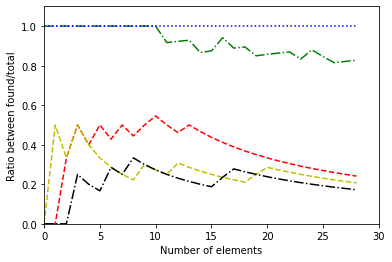
\includegraphics[height=2.5in]{figures/width.png}
\caption{Ratio of anomalies found in the first x using different bit widths for the multiplication. Dataset: Hydice}
  \label{fig:width}
\end{figure}

Como se puede observar en \autoref{fig:width}, ESTO TENGO QUE REPETIRLO.
\\

\subsection{Improving accuracy}
También es necesario crear reglas para desplazar los resultados para mantener la máxima precisión posible sin producir desbordamiento.
\\
Por ejemplo, las divisiones realizadas en el cálculo de la inversa producen números muy pequeños donde la parte fraccionaría resulta relevante para el resultado final. Puesto que esta parte se pierde en la aritmética entera, es necesario multiplicar o desplazar los operandos para producir resultados donde el punto se encuentre desplazado a la izquierda. Estás multiplicaciones se realizarán siempre en potencias de 2, también negativas en el caso de que se requiera decrementar el ancho de bits, ya que resultan triviales de implementar en una FPGA y no gastan recursos.
\\
\\
Estas pruebas se realizaron también en el modelo hardware. Los resultados indicaron que la mayor pérdida de precisión ocurría en el cálculo de la inversa. Por ello se revisó el modelo y se incluyeron desplazamientos en la captura inicial de matrices (en la inicialización en el caso de $A^{-1}$, y en la transferencia a la FPGA en el caso de $A$). También se incluyeron diferentes desplazamientos para cada fase de la inversión.


